% !TeX spellcheck = en_GB
\documentclass[]{subfiles}
\begin{document}
	\section{Definition of a convolution}
	The formal definition of a convolution can be written down as follows:
	\begin{equation*}
		\label{eq:defConvo}
		f(t)\ast g(t) = (f\ast g)(t) = \int_{-\infty}^{\infty} f(\tau) g(t-\tau) d\tau
	\end{equation*}
\subsection{Example for two pulses}
\begin{figure}[h]
	\centering
	\begin{subfigure}{.4\textwidth}
		\begin{center}
				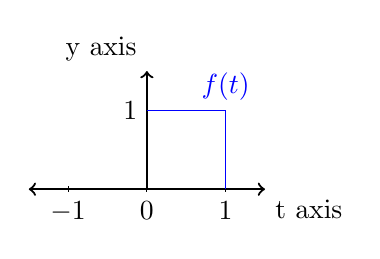
\begin{tikzpicture}
				\centering
				\draw[thick,<->] (-1.5,0) -- (1.5,0) node[anchor=north west] {t axis};
				\draw[thick,->] (0,0) -- (0,1.5) node[anchor=south east] {y axis};
				\foreach \x in {-1,0,1}
				\draw (\x cm,1pt) -- (\x cm,-1pt) node[anchor=north] {$\x$};
				\foreach \y in {1}
				\draw (0,\y cm) -- (0,\y cm) node[anchor=east] {$\y$};
				\draw[blue] (0,1) -- (1,1) node[anchor=south] {$f(t)$}-- (1,0) ;
			\end{tikzpicture}
		\end{center}
	\caption{Function $f(t)$}
	\end{subfigure}%
	\begin{subfigure}{.4\textwidth}
		\begin{center}
					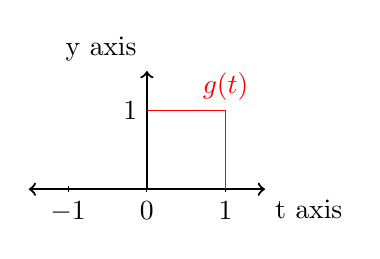
\begin{tikzpicture}
				\centering
				\draw[thick,<->] (-0.5,0) -- (2.5,0) node[anchor=north west] {t axis};
				\draw[thick,->] (1,0) -- (1,1.5) node[anchor=south east] {y axis};
				\foreach \x in {-1,0,1}
				\draw (\x cm +1cm,1pt) -- (\x cm+ 1 cm,-1pt) node[anchor=north] {$\x$};
				\foreach \y in {1}
				\draw (1,\y cm) -- (1,\y cm) node[anchor=east] {$\y$};
				\draw[red] (1,1) -- (2,1) node[anchor=south] {$g(t)$}-- (2,0) ;
			\end{tikzpicture}
		\end{center}
	\caption{Function $g(t)$}
	\end{subfigure}
\caption{The two example pulses before convolution}
\label{fig:convoVoorbeeld}
\end{figure}
The functions in figure \ref{fig:convoVoorbeeld} can be mathematically defined as follows:
\begin{equation*}
	f(t) = g(t) = u(t)-u(t-1)
\end{equation*}
If we apply the definition on these two pulses, we can notice that the function $g(t)$ gets mirrored with respect to the y axis because of the minus sign in the argument as seen in equation \ref{eq:defConvo}. This results in the following figures:  \\

\begin{figure}[h]
	\centering
	\begin{subfigure}{.4\textwidth}
		\begin{center}
			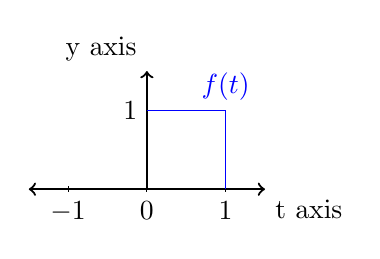
\begin{tikzpicture}
				\centering
				\draw[thick,<->] (-1.5,0) -- (1.5,0) node[anchor=north west] {t axis};
				\draw[thick,->] (0,0) -- (0,1.5) node[anchor=south east] {y axis};
				\foreach \x in {-1,0,1}
				\draw (\x cm,1pt) -- (\x cm,-1pt) node[anchor=north] {$\x$};
				\foreach \y in {1}
				\draw (0,\y cm) -- (0,\y cm) node[anchor=east] {$\y$};
				\draw[blue] (0,1) -- (1,1) node[anchor=south] {$f(t)$}-- (1,0) ;
			\end{tikzpicture}
		\end{center}
		\caption{Function $f(t)$}
	\end{subfigure}%
	\begin{subfigure}{.4\textwidth}
		\begin{center}
			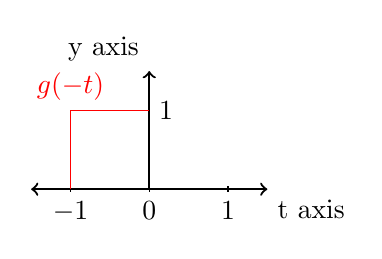
\begin{tikzpicture}
				\centering
				\draw[thick,<->] (-0.5,0) -- (2.5,0) node[anchor=north west] {t axis};
				\draw[thick,->] (1,0) -- (1,1.5) node[anchor=south east] {y axis};
				\foreach \x in {-1,0,1}
				\draw (\x cm +1cm,1pt) -- (\x cm+ 1 cm,-1pt) node[anchor=north] {$\x$};
				\foreach \y in {1}
				\draw (1,\y cm) -- (1,\y cm) node[anchor=west] {$\y$};
				\draw[red] (0,0) -- (0,1) node[anchor=south] {$g(-t)$}-- (1,1) ;
			\end{tikzpicture}
		\end{center}
		\caption{Function $g(-t)$}
	\end{subfigure}
	\caption{Applying the definition}
	\label{fig:convoVoorbeeld2}
\end{figure}
We can now `slide' the function $g(-t)$ over the function $f(t)$. This process is shown in figure \ref{fig:convoSchuiven}.\\

\begin{figure}[h]
	\centering
	\begin{subfigure}{.4\textwidth}
		\begin{center}
			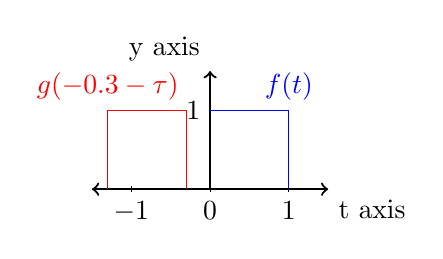
\begin{tikzpicture}
				\centering
				\draw[thick,<->] (-1.5,0) -- (1.5,0) node[anchor=north west] {t axis};
				\draw[thick,->] (0,0) -- (0,1.5) node[anchor=south east] {y axis};
				\foreach \x in {-1,0,1}
				\draw (\x cm,1pt) -- (\x cm,-1pt) node[anchor=north] {$\x$};
				\foreach \y in {1}
				\draw (0,\y cm) -- (0,\y cm) node[anchor=east] {$\y$};
				\draw[blue] (0,1) -- (1,1) node[anchor=south] {$f(t)$}-- (1,0) ;
				\draw[red] (-1.3,0) -- (-1.3,1) node[anchor=south] {$g(-0.3-\tau)$}-- (-0.3,1) -- (-0.3,0) ;
			\end{tikzpicture}
		\end{center}
		\caption{Function $g(-0.3 -\tau)$}
	\end{subfigure}%
		\begin{subfigure}{.4\textwidth}
		\begin{center}
			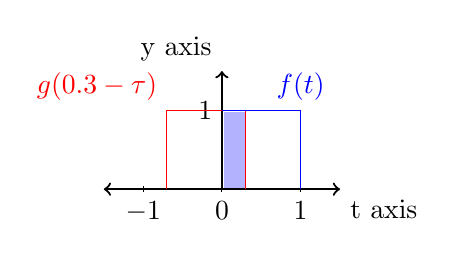
\begin{tikzpicture}
				\centering
				\draw[thick,<->] (-1.5,0) -- (1.5,0) node[anchor=north west] {t axis};
				\draw[thick,->] (0,0) -- (0,1.5) node[anchor=south east] {y axis};
				\foreach \x in {-1,0,1}
				\draw (\x cm,1pt) -- (\x cm,-1pt) node[anchor=north] {$\x$};
				\foreach \y in {1}
				\draw (0,\y cm) -- (0,\y cm) node[anchor=east] {$\y$};
				\draw[red] (-0.7,0) -- (-0.7,1) node[anchor=south east] {$g(0.3-\tau)$}-- (0.3,1) -- (0.3,0) ;
				\draw[blue] (0,1) -- (1,1) node[anchor=south] {$f(t)$}-- (1,0) ;
				\fill[blue!30!white] (0.02,0.02) rectangle (0.29,0.98);
			\end{tikzpicture}
		\end{center}
		\caption{Function $g(0.3 -\tau)$}
	\end{subfigure}%
	\caption{`Sliding' the functions over each other}
	\label{fig:convoSchuiven}
\end{figure}
This process continues until the functions have completely slid over one another. This is the visual interpretation of a convolution.
\newpage
We can compute this convolution as follows:
\begin{align*}
	(f\ast g)(t) &= \int_{-\infty}^{\infty} f(\tau) g(t-\tau) d\tau\\
	&= \int_{-\infty}^{\infty}\left[  u(\tau)-u(\tau-1)\right]  \cdot \left[ u(t-\tau)-u(t-\tau-1)\right] d\tau
\end{align*}
We can now differentiate two cases based on the value of $t$. Figure \ref{fig:tweeGevallen} illustrates these two cases.\\

\begin{figure}[h]
	\centering
	\begin{subfigure}{.4\textwidth}
		\begin{center}
			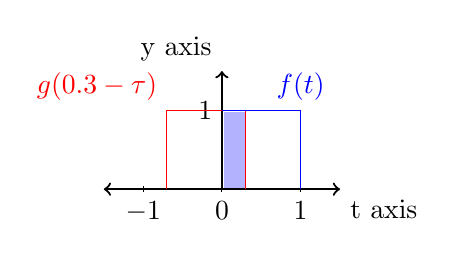
\begin{tikzpicture}
				\centering
				\draw[thick,<->] (-1.5,0) -- (1.5,0) node[anchor=north west] {t axis};
				\draw[thick,->] (0,0) -- (0,1.5) node[anchor=south east] {y axis};
				\foreach \x in {-1,0,1}
				\draw (\x cm,1pt) -- (\x cm,-1pt) node[anchor=north] {$\x$};
				\foreach \y in {1}
				\draw (0,\y cm) -- (0,\y cm) node[anchor=east] {$\y$};
				\draw[red] (-0.7,0) -- (-0.7,1) node[anchor=south east] {$g(0.3-\tau)$}-- (0.3,1) -- (0.3,0) ;
				\draw[blue] (0,1) -- (1,1) node[anchor=south] {$f(t)$}-- (1,0) ;
				\fill[blue!30!white] (0.02,0.02) rectangle (0.29,0.98);
			\end{tikzpicture}
		\end{center}
		\caption{ $t\leq 1$}
	\end{subfigure}%
	\begin{subfigure}{.4\textwidth}
		\begin{center}
			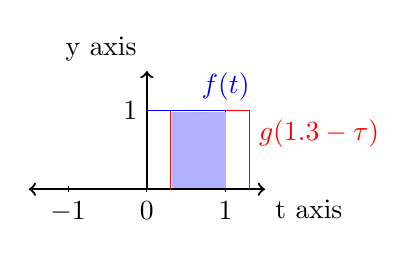
\begin{tikzpicture}
				\centering
				\draw[thick,<->] (-1.5,0) -- (1.5,0) node[anchor=north west] {t axis};
				\draw[thick,->] (0,0) -- (0,1.5) node[anchor=south east] {y axis};
				\foreach \x in {-1,0,1}
				\draw (\x cm,1pt) -- (\x cm,-1pt) node[anchor=north] {$\x$};
				\foreach \y in {1}
				\draw (0,\y cm) -- (0,\y cm) node[anchor=east] {$\y$};
				\draw[red] (0.3,0) -- (0.3,1) -- (1.3,1) node[anchor=north west] {$g(1.3-\tau)$}-- (1.3,0) ;
				\draw[blue] (0,1) -- (1,1) node[anchor=south] {$f(t)$}-- (1,0) ;
				\fill[blue!30!white] (0.32,0.02) rectangle (1,0.98);
			\end{tikzpicture}
		\end{center}
		\caption{$t\geq 1$}
	\end{subfigure}%
	\caption{Two cases}
	\label{fig:tweeGevallen}
\end{figure}
We can now divide the process in figure \ref{fig:tweeGevallen} into three different stages using elementary integrals. 
\begin{align*}
	(f\ast g)(t) &= \int_{0}^{t}1d\tau = t \quad&\text{voor}\quad 0\leq t\leq 1\\
	(f\ast g)(t) &= \int_{t-1}^{1}1d\tau = -t+2 \quad&\text{voor} \quad1\leq t\leq 2\\
	(f\ast g)(t) &= 0 \quad&\text{voor} \quad t\leq 0\vee t\geq 2
\end{align*}
We can graphically represent these results as follows: 
\begin{center}
	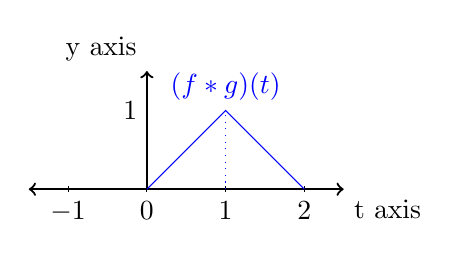
\begin{tikzpicture}
		\centering
		\draw[thick,<->] (-1.5,0) -- (2.5,0) node[anchor=north west] {t axis};
		\draw[thick,->] (0,0) -- (0,1.5) node[anchor=south east] {y axis};
		\foreach \x in {-1,0,1,2}
		\draw (\x cm,1pt) -- (\x cm,-1pt) node[anchor=north] {$\x$};
		\foreach \y in {1}
		\draw (0,\y cm) -- (0,\y cm) node[anchor=east] {$\y$};
		\draw[blue] (0,0) -- (1,1) node[anchor=south] {$(f\ast g)(t)$}-- (2,0) ;
		\draw[blue, dotted] (1,0) -- (1,1);
	\end{tikzpicture}
\end{center}
\end{document}
